\documentclass[conference]{IEEEtran}
\IEEEoverridecommandlockouts
% The preceding line is only needed to identify funding in the first footnote. If that is unneeded, please comment it out.
%\usepackage{cite}
%\usepackage{amsmath,amssymb,amsfonts}
%\usepackage{algorithmicx}
\usepackage{graphicx}
\usepackage{subcaption}
\usepackage{textcomp}
%\usepackage{xcolor}
\def\BibTeX{{\rm B\kern-.05em{\sc i\kern-.025em b}\kern-.08em
    T\kern-.1667em\lower.7ex\hbox{E}\kern-.125emX}}
\begin{document}

\title{Networked Predictive Control\\
%{\footnotesize \textsuperscript{*}Note: Sub-titles are not captured in Xplore and
%should not be used}
%\thanks{Identify applicable funding agency here. If none, delete this.}
}

\author{\IEEEauthorblockN{ Freddy Pesantez}
\IEEEauthorblockA{
freddy.pesantez@uchile.cl}
%\and
%\IEEEauthorblockN{ Daniel Baeza}
%\IEEEauthorblockA{
%dabaeza@uchile.cl}
%\and
%\IEEEauthorblockN{3\textsuperscript{rd} Given Name Surname}
%\IEEEauthorblockA{\textit{dept. name of organization (of Aff.)} \\
%\textit{name of organization (of Aff.)}\\
%City, Country \\
%email address}
}

\maketitle

\begin{abstract}
En el mundo moderno los sistemas de control distribuido cada vez son más comunes, gracias al avance tecnológico. Un punto crucial para que  
\end{abstract}

\begin{IEEEkeywords}
Reconocimiento de imágenes, Imágenes de marcas.
\end{IEEEkeywords}

\section{Introduction}
En el mundo actual es muy común que las empresas utilicen algún tipo de imagen llamativa para su identificación en el mercado, de forma tal que les permita ser reconocidos fácilmente en el mercado. Estas imágenes tienen mucho valor porque les permite posicionarse de alguna manera en las preferencias de los usuarios, por lo tanto el uso de ellas constituye en factor importante en un ambiente de mercado.

Sin embargo, no es difícil imaginarse que el número actual de estas imágenes de las marcas se ha ido incrementado enormemente con el tiempo, y las bases de datos actuales son muy grandes. Por lo mencionado antes, estas imágenes están sujetas a derechos de autor en los países.

<<<<<<< HEAD
Para el registro de una nueva imagen se debe verificar que no existan otras imágenes lo suficientemente parecidas como para que exista confusión por un lado y para que no se violen los derechos de autor. 
=======
Sin embargo, el número actual de logos se ha ido incrementado enormemente con el tiempo, haciendo mas difícil el trabajo de los expertos en las oficinas de registro. 

Por esta razones, en visión computacional, el reconocimiento de marcas ha tenido un creciente interés. En la actualidad no existen metodologías que tengan tasas de clasificación superiores a la de un experto, pero si han contribuido a facilitar el trabajo de estas personas.

En este trabajo se propone analizar el desempeño de tres de los métodos mas utilizados actualmente para el reconocimiento de marcas. El primero intenta encontrar patrones locales en los logos que permitan su discriminación. El segundo se basa en en el análisis de componentes principales espectral, extrayendo así características generales del logo. Por último se implementará un método de clasificación basado en la forma de las marcas.

Estos métodos serán puestos a prueba con un subconjunto de imágenes extraídas de la base de logos mas grande actualmente, orientada a medir desempeño en metodologías de detencción y reconocimineto de marcas.

El presente informe se estructura de la siguiente forma. A continuación se muestra un estado del arte en el tema de reconocimiento de marcas desde el punto de vista de visión computacional. Posteriormente, en este reporte se realiza una descripción de los métodos seleccionados. Finalmente se describe la base de datos a utilizar, justificando su uso mediante comparaciones con el resto de las bases de datos disponibles.
>>>>>>> 00b9f2fa05bc5d45654137357ff7d40941774d74


\section{Estado del Arte}
La primera forma en que se enfrentó el reconocimiento y detección de marcas fue a tráves de una persona, la cual "memoriza" una imagen y busca similitues en una base de datos. Esta solución, al tener bases de datos de miles de logos, comprende un tiempo muy largo de trabajo por parte de los expertos, además de errores de interpretación o sesgos que dependen de cada persona.
En visión computacional, resulta muy desafiante este tipo de problemas ya que se necesita detección y clasificación de elmentos muy diversos en color, forma, tamaño, iclusión de cateres y/o palabras, etc. En este mismo sentido, resulta necesario la construcción de medidas de similitud o distancia entre distintas imágenes de marcas.

En la actualidad existen varias metodologías desarrolladas para el reconocimiento y detección de logos en imágenes basadas en visión computacional. Un estudio del desempeño de las metodologías con mejor desempeño fue hecho por Tursun et al. \cite{metuV2}. En esta publicación los autores hacen comparaciones entre metodologías basadas en extracción de características con apoyo experto[\cite{bowd}, \cite{colorHist}, \cite{GIST}, \cite{kpoint}, \cite{LBP}, \cite{shape}] y las basadas en aprendizaje de máquina utilizando redes convolucionales[\cite{cnn1}, \cite{cnn2}]. 

El resultado del estudio hecho por Tursun et al. \cite{metuV2} concluye un desempeño sobresaliente de los métodos basados en redes convolucionales, sin embargo, aún no alcanzan una tasa de clasificación comparable con un humano experto. 

Además de los resultados de desempeño de las distintas metodologías, en el trabajo de Tursun et al. \cite{metuV2} se presenta la segunda versión de la librería METU. Esta librería, cuya primera versión fue desarrollada por Tursun \& Kalkan \cite{metuV1}, es actualmente la base de datos mas diversa y numerosa de todas las utilizadas en investigaciones relacionadas con reconocimiento y detección de marcas en imágenes. Mas detalles de esta base de datos se muestran en secciones posteriores de este informe. 


\section{Metodologías seleccionadas}
A continuación se describen las metodologías seleccionadas para medir sus desempeños en el problema de reconocimiento y detección de logos. Además, se probará el desempeño bajo tres métricas: euclidiana, similitud coseno y distancia manhattan.

\subsection{Caracter\'isticas de la textura: Patrones locales binarios (LBP)}

Un algoritmo que se ha demostrado es muy eficiente para esta tarea es conocido por sus siglas en inglés como LBP\cite{LBP}. Este algoritmo lo que hace es establecer simulitud entre pixeles basados en vecindario. La comparación se realiza mediante el índice calculado con la siguiente ecuación,

\ref{eq:distLBP} 
	\begin{equation}
	L_{P,R} = \sum_{p=0}^{P-1} s{(g_p - g_c)}^{{2}^p}
	\label{eq:distLBP}
\end{equation}

Donde $P$ es la cuenta de los vecinos en un círculo de radio $R$, y $g_p$ y $g_c$ son intensidades de el pixel p y el pixel central respectivamente.

\subsection{Características Generales: GIST}
GIST es un algoritmo que extrae características generales del entorno en el cual está la imagen. Está basado en el calculo de componentes principales de la energía espectral. En el trabajo hecho por Douze et al. \cite{GIST} muestran el desempeño de GIST como herramienta para el control de propiedad intelectual. En este estudio muestra tener un mejor desempeño que algoritmos usados comúnmente usados como detección de texto BoVW \cite{bowd} con descriptores locales como SIFT \cite{kpoint}.



\subsection{Forma general de la imagen}

La forma de la imagen es quizás uno de las carácterísticas más importantes en la detección y reconocmiento de logos. El método propuesto por \cite{shape} tiene un buen desempeño en este tipo de problemas.

La metodología general de extracción de formas es la siguiente:

\begin{enumerate}
\item{Muestrear uniformemente n puntos de la parte interior y exterior de la forma}

\item{Asignar un histograma tipo log-polar a cada muestra}

\item{De acuerdo a la localización de las muestras en cada histograma logarítmico, generar n vectores del contorno de la forma}
\end{enumerate}


\section{Base de datos METU}
La base de datos METU es introducida por Tursun \& Kalkan \cite{metuV1}. LA base de datos METU Posee mas de 900.000 imágenes de logos en distintas resoluciones. La tabla \ref{tab:MATUFeatures} muestra las características de METU.
\begin{table}[h!]
	\caption{Características de base de datos MATU}
	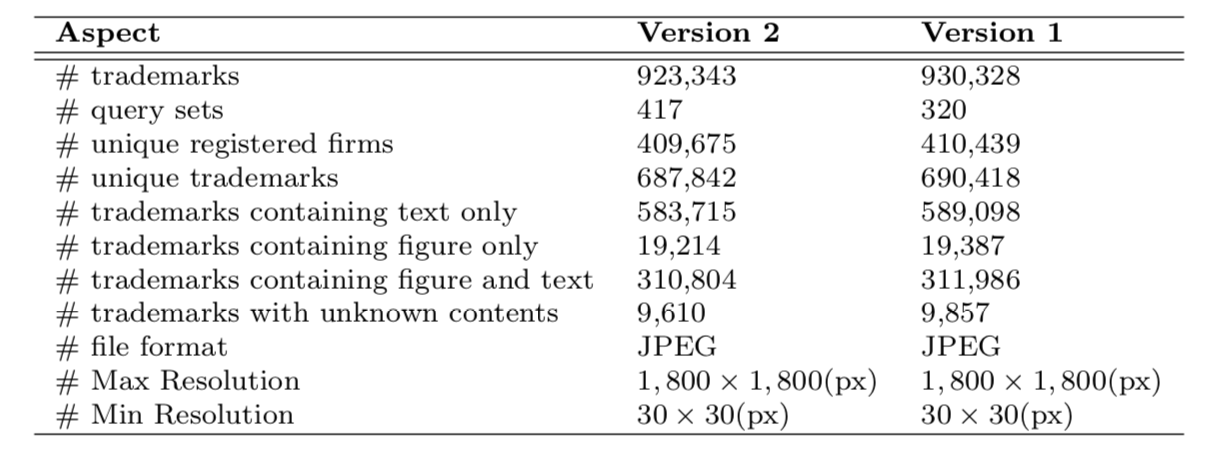
\includegraphics[width=8cm]{images/caracteristicasMatu}
	\label{tab:MATUFeatures}
\end{table}

En el estudio hecho por Tursun et al. \cite{metuV2} se muestra además que METU es la base de datos mas numerosa y refinada entre las usadas actualmente en investigación. La tabla \ref{tab:datasetComparison} muestra una comparación entre las distintas bases de datos usadas en reconocimiento de marcas.
\begin{table}[h!]
	\caption{Comparación entre distintas bases de datos}
	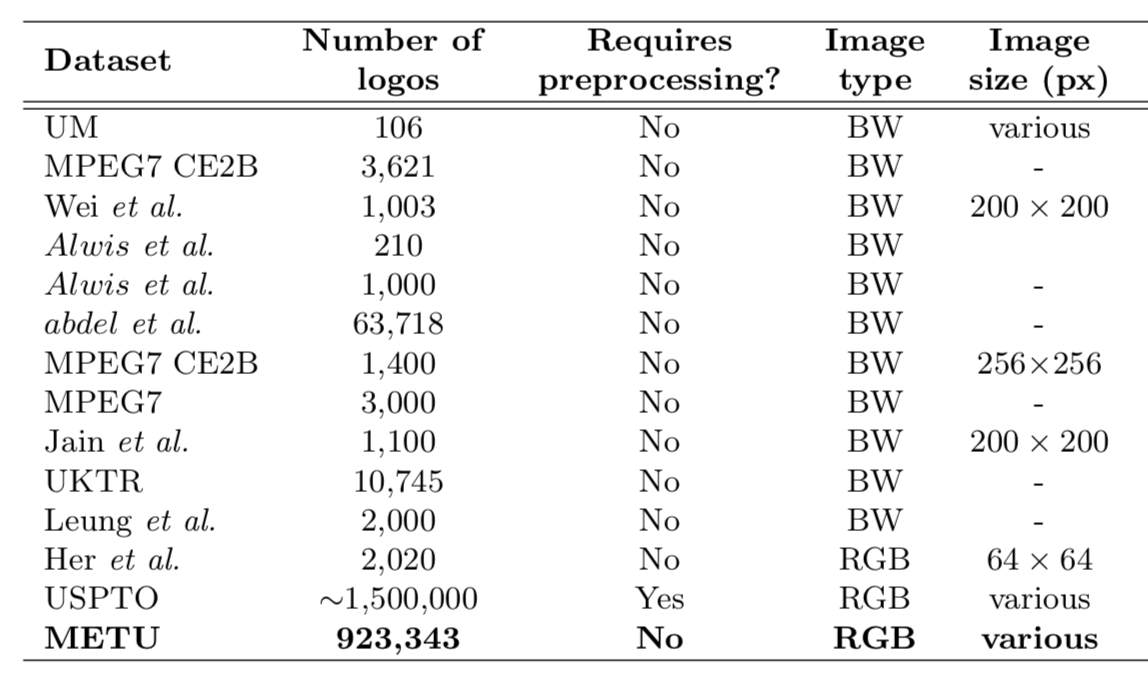
\includegraphics[width=8cm]{images/comparasciondataset}
	\label{tab:datasetComparison}
\end{table}

Para este proyecto METU será la base de datos en que se probarán las metodologías seleccionadas. Algunos ejemplos de logos incluidos en la base de datos METU se muestran en las Figura \ref{fig:logosMatu}.

\begin{figure}[h!]
\centering
	\begin{subfigure}[b]{0.8\linewidth}
		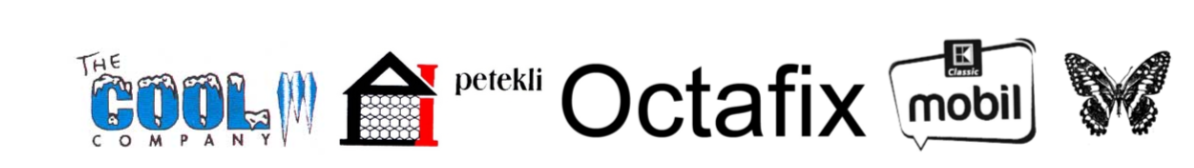
\includegraphics[width=\linewidth]{images/metudataset.png}
		\caption{Ejemplos de logos entrenamiento de METU}
	\end{subfigure}

  	\begin{subfigure}[b]{0.8\linewidth}
		
\includegraphics[width=\linewidth]{images/queriesmetu2}
		\caption{Ejemplos de logos de validación de METU}
  	 \end{subfigure}
  	\caption{Ejemplos de logos en base de datos METU}
  	\label{fig:logosMatu}
\end{figure} 

\begin{thebibliography}{00}

\bibitem{b1} Tursun, O., Aker, C., \& Kalkan, S. (2017). A large-scale dataset and benchmark for similar trademark retrieval. arXiv preprint arXiv:1701.05766.

\bibitem{b2} Simonyan, K., \& Zisserman, A. (2014). Very deep convolutional networks for large-scale image recognition. arXiv preprint arXiv:1409.1556.

\bibitem{b3} Szegedy, C., Liu, W., Jia, Y., Sermanet, P., Reed, S., Anguelov, D., ... \& Rabinovich, A. (2015). Going deeper with convolutions. In Proceedings of the IEEE conference on computer vision and pattern recognition (pp. 1-9).

\bibitem{b5} Tursun, O., ,\& Kalkan, S. (2015, May). Metu dataset: A big dataset for benchmarking trademark retrieval. In Machine Vision Applications (MVA), 2015 14th IAPR International Conference on (pp. 514-517). IEEE.

\end{thebibliography}


\end{document}
